\section{Construction of the parser}
	In this section we will describe how one can construct a parser from a EBNF, but first we will describe what a parser is and how it works.
	
	\subsection{Parsing strategies}
		The job of a parser is to check if a program is correct and 
		to determine the structure of the program, the latter is usually done by constructing a syntax tree.
		There are two common ways of checking this {\it Bottom-up Parsing} and {\it Top-Down Parsing}.
		
		\subsubsection*{Bottom-up Parsing}
			This way of parsing takes simple structures and combining them to more complex structures.
			We call this type of parsing for {\it LR parsing} because we read the text from the left and reduces to the right.
			\begin{figure}[H]
				\centering
				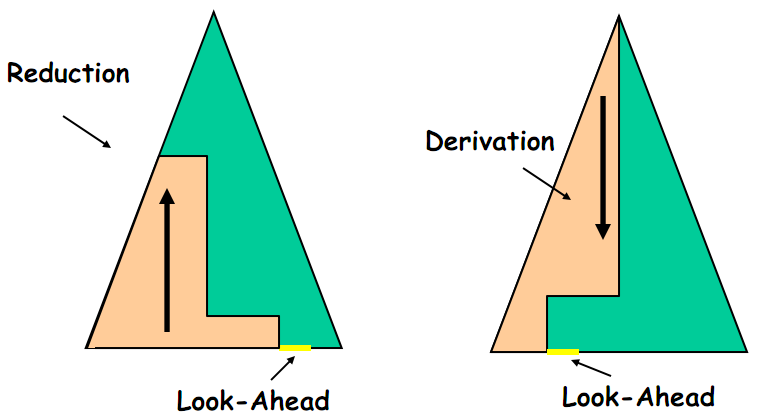
\includegraphics[width=0.8\textwidth]{rapport/2/figures/parsestrat.png}
				\caption{Left figure bottom-up parsing - Right figure top-down parsing}\label{fig:lrparse}
			\end{figure}
			
		\subsubsection*{Top-down Parsing}
			Top-down parsing starts from the complex structures, and breaks them down into smaller parts.
			We call this type of parsing for {\it LL parsing} because we read the text from the left and make derivations to the left.
		
		\subsubsection*{Strengths and weaknesses}
			The most commonly used parsing strategy of the two is LR parsing, the reason for this is because it's faster than LL parsing.
			However a LR parser is much bigger is 
			In this project, however we have chosen to make a LL parser because it's easy to make by hand. The type of LL parser we made is called
			a recursive descent parser.
			
	\subsection{Creating a recursive descent parser}
		A recursive descent parser is a LL parser which works by recursively going through the program.
		To construct this type of parser a EBNF is required and here is how it is made:
		\begin{enumerate}
			\item Make a scanner for reading chars and identifying them as terminals.
			\item Make a parse method for each non-terminal in the EBNF.
			\item Make a method that can accept terminals.
			\item In each of the parse method accept terminals and/or call other parse methods.
		\end{enumerate}		
	
	%leder ikke så godt synes jeg :/	
		%This chapter was about parsing, now to Scope Rules (Contextual analysis)
		%A parser is an important tool to make the WAR interpreter, and now to defining the scope rules and type checking in the contextual analysis part.		
		
		
		